%%%%%%%%%%%%%%%%%%%%%%%%%%%%%%%%%%%%%%%%%
% Jacobs Portrait Poster
% LaTeX Template
% Version 1.0 (31/08/2015)
% (Based on Version 1.0 (29/03/13) of the landscape template
%
% Created by:
% Computational Physics and Biophysics Group, Jacobs University
% https://teamwork.jacobs-university.de:8443/confluence/display/CoPandBiG/LaTeX+Poster
% 
% Further modified by:
% Nathaniel Johnston (nathaniel@njohnston.ca)
%
% Portrait version by:
% John Hammersley
%
% The landscape version of this template was downloaded from:
% http://www.LaTeXTemplates.com
%
% License:
% CC BY-NC-SA 3.0 (http://creativecommons.org/licenses/by-nc-sa/3.0/)
%
%%%%%%%%%%%%%%%%%%%%%%%%%%%%%%%%%%%%%%%%%

%----------------------------------------------------------------------------------------
%	PACKAGES AND OTHER DOCUMENT CONFIGURATIONS
%----------------------------------------------------------------------------------------

\documentclass[final,xcolor=x11names,table]{beamer}

\usepackage[scale=1.24, size=a1]{beamerposter} % Use the beamerposter package for laying out the poster
\usepackage{tikz}
\usepackage{lipsum}
\usepackage[utf8]{inputenc}
\usepackage[english]{babel}
\usepackage[TS1,T1]{fontenc}
% \usepackage{enumerate}
% \usepackage{fourier,heuristica}
% \usepackage{array, booktabs}
\usepackage{caption} % define caption
\usepackage{graphicx}  % Required for including images
\usepackage{booktabs} % Top and bottom rules for tables
\usepackage{standalone}
\DeclareCaptionFont{blue}{\color{LightSteelBlue3}}
\usetheme{confposter} % Use the confposter theme supplied with this template

\setbeamercolor{block title}{fg=ngreen,bg=white} % Colors of the block titles
\setbeamercolor{block body}{fg=black,bg=white} % Colors of the body of blocks
\setbeamercolor{block alerted title}{fg=white,bg=dblue!70} % Colors of the highlighted block titles
\setbeamercolor{block alerted body}{fg=black,bg=dblue!10} % Colors of the body of highlighted blocks
% Many more colors are available for use in beamerthemeconfposter.sty

%-----------------------------------------------------------
% Define the column widths and overall poster size
% To set effective sepwid, onecolwid and twocolwid values, first choose how many columns you want and how much separation you want between columns
% In this template, the separation width chosen is 0.024 of the paper width and a 4-column layout
% onecolwid should therefore be (1-(# of columns+1)*sepwid)/# of columns e.g. (1-(4+1)*0.024)/4 = 0.22
% Set twocolwid to be (2*onecolwid)+sepwid = 0.464
% Set threecolwid to be (3*onecolwid)+2*sepwid = 0.708

\newlength{\sepwid}
\newlength{\onecolwid}
\newlength{\twocolwid}
\newlength{\threecolwid}

\setlength{\paperwidth}{36in} % A0 width: 46.8in
\setlength{\paperheight}{48in} % A0 height: 33.1in
\setlength{\sepwid}{0.024\paperwidth} % Separation width (white space) between columns
\setlength{\onecolwid}{0.22\paperwidth} % Width of one column
\setlength{\twocolwid}{0.464\paperwidth} % Width of two columns
\setlength{\threecolwid}{0.708\paperwidth} % Width of three columns

\setlength{\topmargin}{-0.7in} % Reduce the top margin size
%-----------------------------------------------------------

% custom command
\newcommand{\foo}{\color{LightSteelBlue3}\makebox[0pt]{\textbullet}\hskip-0.5pt\vrule width 1pt\hspace{\labelsep}}
%----------------------------------------------------------------------------------------
%	TITLE SECTION 
%----------------------------------------------------------------------------------------

\title{Cross Plaform Application Development} % Poster title

\author{Course: IERG4999 \and Student Name: Doria Tang\\Supervisor: Prof. Kehuan Zhang} % Author(s)

\institute{Dept. of Information Engineering, The Chinese University of Hong Kong} % Institution(s)

\setbeamertemplate{headline}{
 \leavevmode
  \begin{columns}[T]
    \begin{column}{0.25\linewidth}
        \vskip1cm
        \hskip1cm
        
\includegraphics[width=\linewidth]{cuhk.png}
    \end{column}
        \begin{column}{.93\linewidth}
         \vskip2cm
         \centering
         \usebeamercolor{title in headline}{\color{jblue}\huge{\textbf{\inserttitle}}\\[0.5ex]}
         \usebeamercolor{author in headline}{\color{fg}\Large{\insertauthor}\\[1ex]}
         \usebeamercolor{institute in headline}{\color{fg}\large{\insertinstitute}\\[1ex]}
         \vskip1cm
        \end{column}
    \begin{column}{0.25\linewidth}
        \vskip1cm
        
\includegraphics[width=\linewidth]{cuhk.png}
        \hskip1cm
    \end{column}        
   \vspace{1cm}
  \end{columns}
 \vspace{0.3in}
 \hspace{0.5in}\begin{beamercolorbox}[wd=47in,colsep=0.15cm]{cboxb}\end{beamercolorbox}
 \vspace{0.1in}
}
%----------------------------------------------------------------------------------------

\begin{document}

\addtobeamertemplate{block end}{}{\vspace*{2ex}} % White space under blocks
\addtobeamertemplate{block alerted end}{}{\vspace*{2ex}} % White space under highlighted (alert) blocks

\setlength{\belowcaptionskip}{1.5ex} % White space under figures
\setlength\belowdisplayshortskip{1ex} % White space under equations

\begin{frame}[t] % The whole poster is enclosed in one beamer frame

\begin{columns}[t] % The whole poster consists of three major columns, the second of which is split into two columns twice - the [t] option aligns each column's content to the top

\begin{column}{\sepwid}\end{column} % Empty spacer column

\begin{column}{\onecolwid} % The first column
% \begin{column}{\colwidth}

\begin{alertblock}{Objectives}
\begin{itemize}
\item To create an online anonymous platform that allows users to express their opinions freely.
\item To provide an informative platform that encourages users to explore different books.
\item To develop a small community that users can meet people who share similar interests.
\end{itemize}
\end{alertblock}

\begin{block}{Introduction}
    \textbf{Overview.\space}The project is based on a cross-platform application framework that encourages students to exchange their books and ideas on an online platform.\\
    \textbf{Motivation.\space} This project aimed to solve two major problems:
    \begin{itemize}
        \item Allow students to meet more friends through the use of social media application. \cite{covid19:2022jd,Parlak:2012qr}
        \item Address the problem of wasted textbooks by encouraging them to exchange the used books.
    \end{itemize}
    \textbf{Technical Background.\space}The application is targeted to deploy on iOS and Android.
    \begin{itemize}
        \item Frontend: Flutter framework + Dart language \cite{Flutter:Documentation}
            \begin{itemize}
                \item[--] Only a single codebase is used
                \item[--] Code is rendered as widgets in the element tree to represent the current state of user interface
                \item[--] The rendering tree is then used to generate a platform-agnostic Skia canvas
                \item[--] GPU renders the UI to the screen to achieve cross-platform effect
            \end{itemize}
            \begin{figure}
                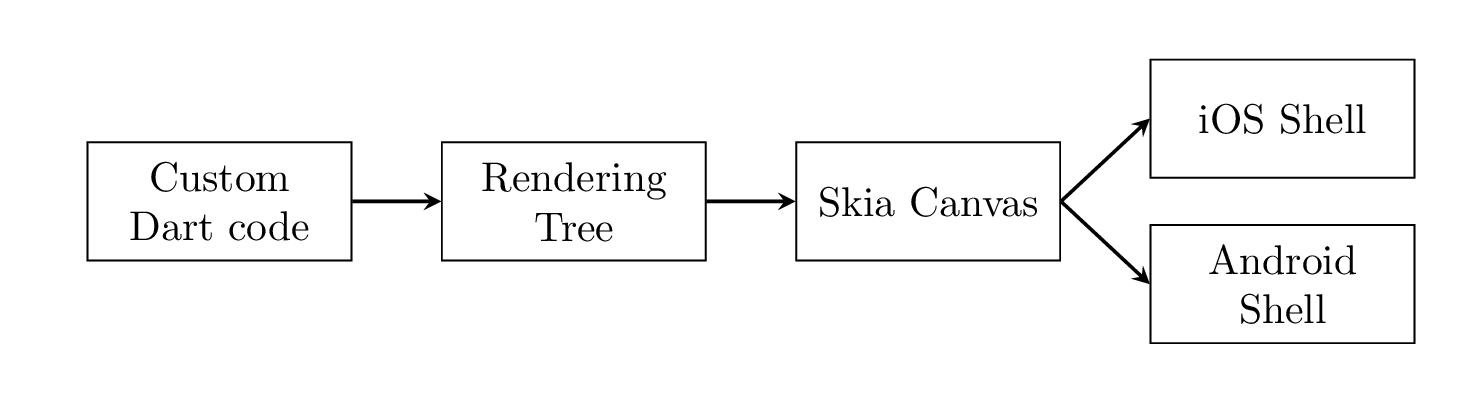
\includegraphics[width=\linewidth]{rendering.png}
                \caption{Flutter rendering process}
            \end{figure}
        \vspace{-2.3cm}
        \item Backend: Node.js server to create various APIs
        \item Database: MongoDB to create non-relational documents \cite{MongoDB:Documentation}
        \begin{figure}
            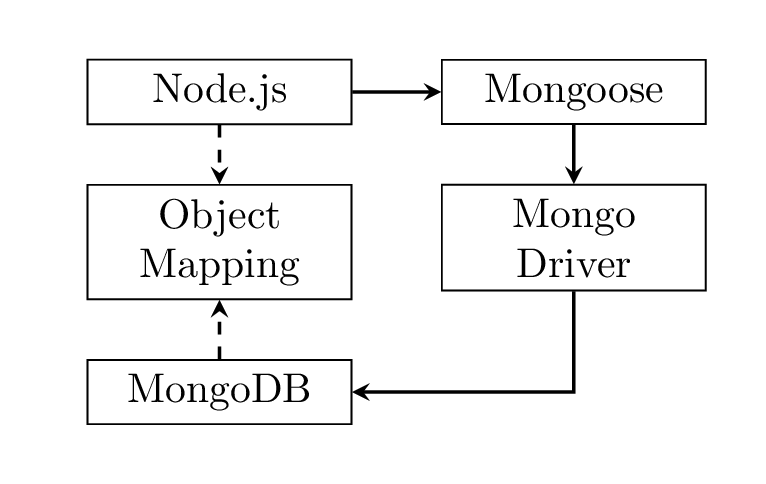
\includegraphics[width=0.8\linewidth]{backend.png}
            \caption{Nodejs and MongoDB relations}
        \end{figure}
        \vspace{-2.3cm}
        Node.js uses the Mongoose package as the driver to communicate with MongoDB and perform various actions. The Schema and models are defined using Mongoose API and send the queries back to the server in JSON-format.
    \end{itemize}
\end{block}

\end{column} % End of first column

\begin{column}{\sepwid}\end{column} % Empty spacer column

\begin{column}{\twocolwid} % second column

\begin{block}{Methodology}
The application consists of three main parts: the frontend application, the backend server, and the database. The three-layer architecture allows for separations for the whole application, so that it allows for easier maintenance and performs independent updates on different components.\\
\begin{figure}
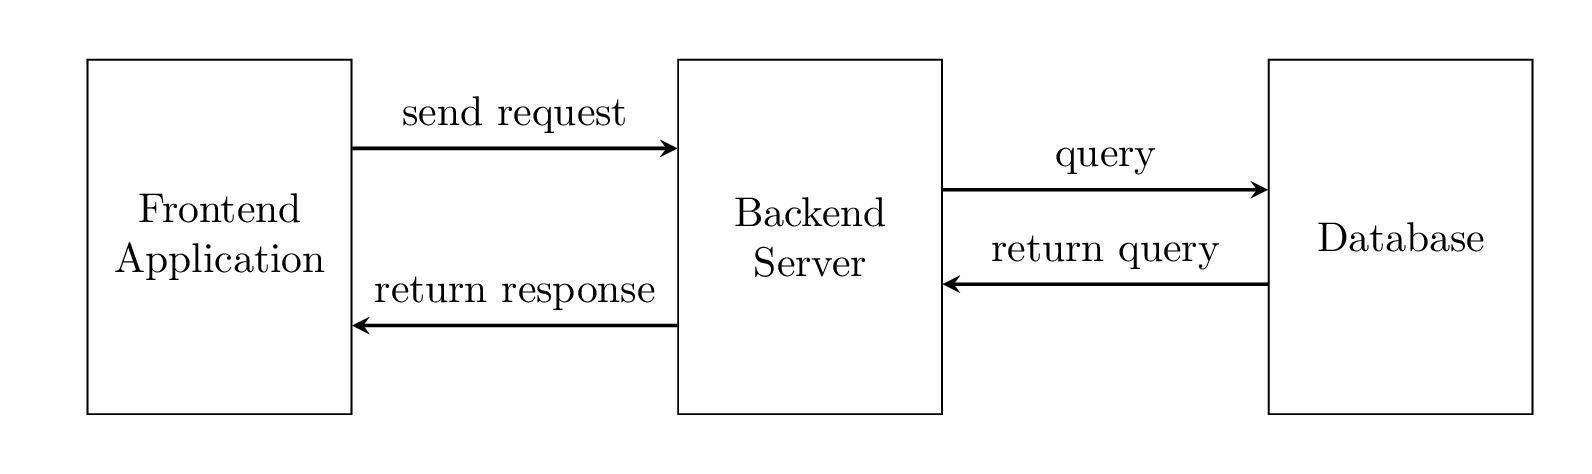
\includegraphics[width=0.8\linewidth]{app_architecture.png}
\caption{Application Architecture}
\end{figure}
\vspace{-1.0cm}
\textbf{Frontend Application.\space}The frontend handles user interaction and information display. It focuses on:
\begin{itemize}
    \item \textbf{User-friendly interface:\space}night mode, responsive screen etc.
    \item \textbf{User actions:\space}uploading books, leaving comments etc.
    \item \textbf{Third-party API implementations:\space}ChatGPT, New York Times API
\end{itemize}
\textit{\small**This part will be presented in the live demo.}\\
% \begin{figure}[!htb]
%     \minipage{0.2\textwidth}%
%         \centering
%         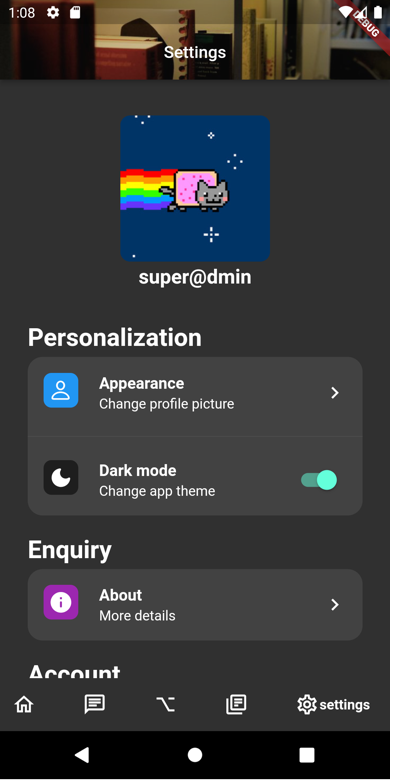
\includegraphics[width=0.7\linewidth]{night.png}
%         % \caption{A really Awesome Image}\label{fig:awesome_image1}
%     \endminipage\hfill
%     \minipage{0.2\textwidth}%
%         \centering
%         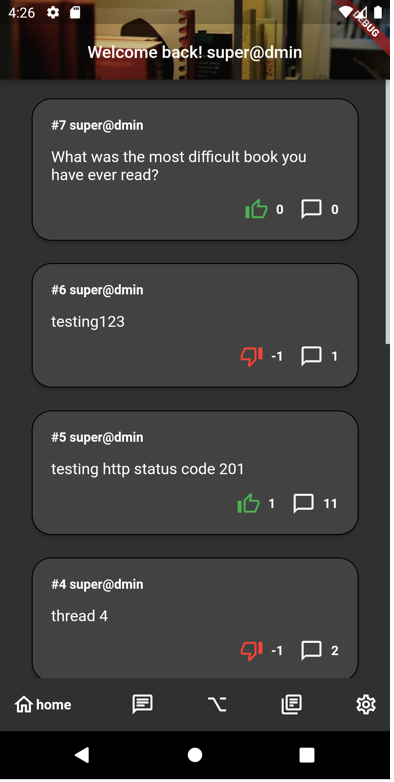
\includegraphics[width=0.7\linewidth]{homepage.png}
%         % \caption{A really Awesome Image}\label{fig:awesome_image2}
%     \endminipage\hfill
%     \minipage{0.2\textwidth}%
%         \centering
%         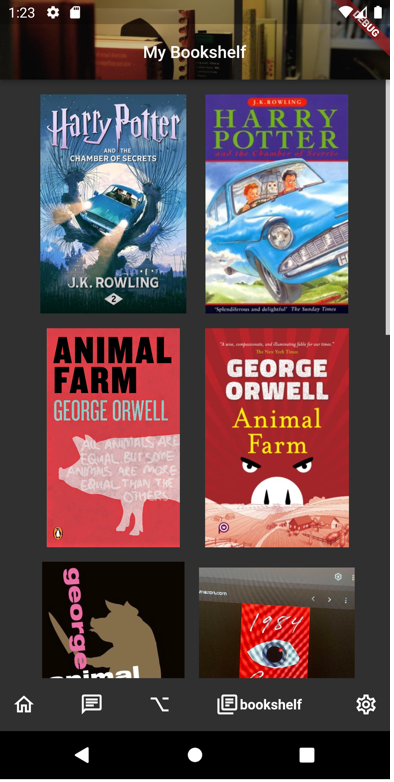
\includegraphics[width=0.7\linewidth]{bookshelf.png}
%         % \caption{A really Awesome Image}\label{fig:awesome_image3}
%     \endminipage\hfill
%     \minipage{0.2\textwidth}%
%         \centering
%         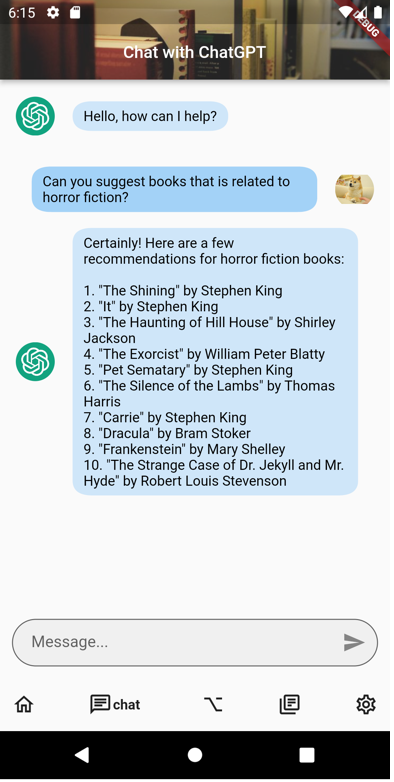
\includegraphics[width=0.7\linewidth]{chatgpt.png}
%         % \caption{A really Awesome Image}\label{fig:awesome_image3}
%     \endminipage\hfill
%     \minipage{0.2\textwidth}%
%         \centering
%         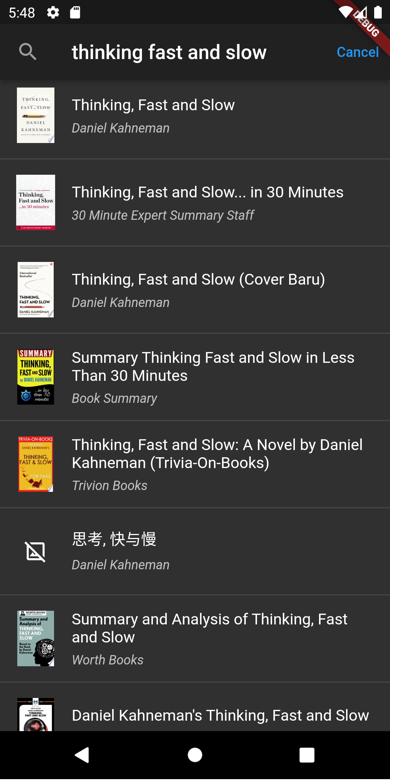
\includegraphics[width=0.7\linewidth]{search.png}
%         % \caption{A really Awesome Image}\label{fig:awesome_image3}
%     \endminipage\hfill
%     \caption{Some Frontend UIs}
% \end{figure}
\textbf{Backend Server.\space}Backend server connects frontend to database and handles user data. The API calls are categorized as:\\
\begin{itemize}
    \item \textbf{User:\space}manage user information, such as changing account password.
    \item \textbf{Thread:\space}manage discussion threads, such as fetching content from all the threads, creating threads, giving likes or dislikes.
    \item \textbf{Comment:\space}manage comments, such as fetching information of all the comments in a thread, creating comments, editing comments.
    \item \textbf{Book:\space}manage the book uploading action, such as adding book picture and retreiving book information. 
\end{itemize}
\textbf{Database.\space}The non-relational database can store different data types in the documents. A query doesn’t have to view several tables to find the desired data, which leads to a better performance compared to traditional database.
\begin{figure}
    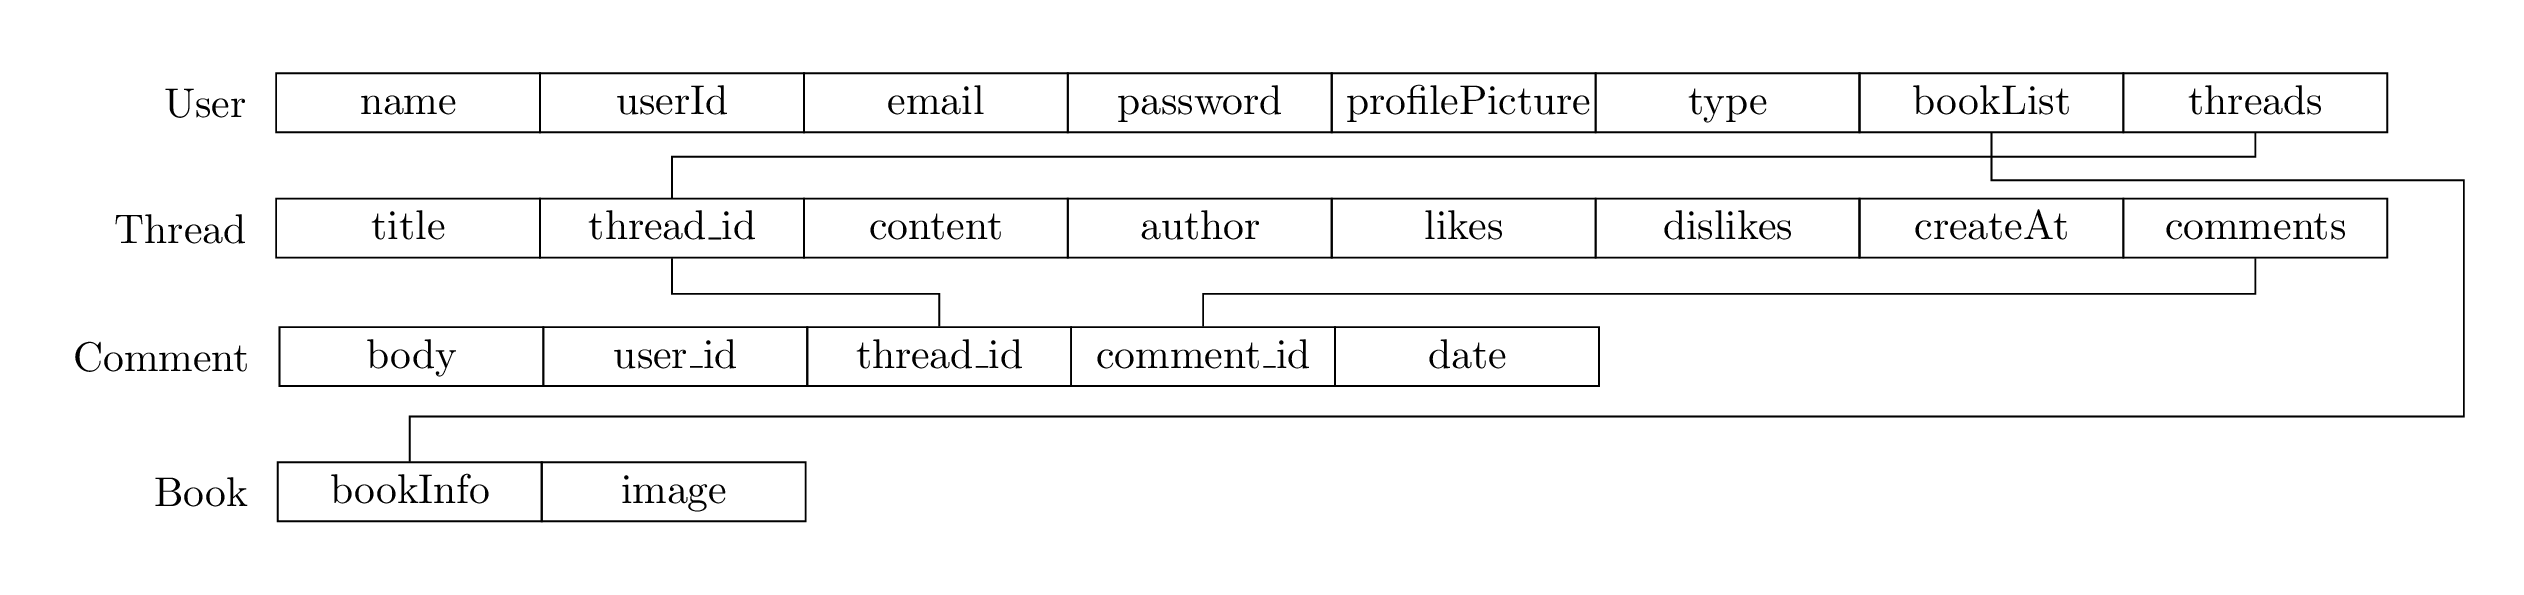
\includegraphics[width=1\linewidth]{database.png}
    % \documentclass[border=5mm, convert]{standalone}
\usepackage{tikz}
\usetikzlibrary{shapes,arrows}
\usetikzlibrary{arrows.meta,positioning}

\begin{document}
% all other packages and stuff you need for the picture
% styles
\tikzstyle{arrow} = [thick,->,>=stealth]
\tikzstyle{box} = [rectangle, 
minimum width=0.5cm, 
minimum height=3cm,
text centered, 
draw=black,text width=2cm]

\begin{tikzpicture}[node distance=5cm] % your picture code
\node (app) [box] {Frontend Application};
\node (server) [box, right of=app] {Backend Server};
\node (database) [box, right of=server] {Database};

\draw [arrow]([yshift=0.75cm]app.east) coordinate (aux1) -- node[anchor=south]{send request} (aux1 -| server.west);
\draw [arrow]([yshift=0.4cm]server.east) coordinate (aux1) -- node[anchor=south]{query} (aux1 -| database.west);
\draw [arrow]([yshift=-0.4cm]database.west) coordinate (aux2) -- node[anchor=south]{return query} (aux2 -| server.east); 
\draw [arrow]([yshift=-0.75cm]server.west) coordinate (aux2) -- node[anchor=south]{return response} (aux2 -| app.east); 

\end{tikzpicture}
\end{document}
    \caption{Relations between Documents in MongoDB}
\end{figure}
\vspace{-1.0cm}
Documents in MongoDB are linked with their object ID. This allows developers to modify the database dynamically.
\end{block}

\begin{block}{Testing}
% attach UAT testing result
\textbf{User Acceptance Tests:}\\
The purpose of the test is to check whether the UI widgets are running properly before putting to production environment.
% attach a table
\begin{table}[ht]
    \centering
    \begin{tabular}[t]{lccc}
        \hline
        &User Interface related&User Actions&Third-Party APIs\\
        \hline
        Passed&7&24&4\\
        Failed&1&7&2\\
        Total&8&31&6\\
        \hline
    \end{tabular}
    \caption{User Acceptance Tests Evaluation}
\end{table}%
The majority of the failed tests were attributed to UI components incorrectly displaying information, with some of them showing incorrect updates.\\
\indent $\rightarrow$ \textit{Improvements: automation testing, invite more testers}\\

\textbf{Functional Tests:}\\
The functional test for the backend server's API is conducted using Postman and involves running test script to verify the accuracy of the response structure, such as response status code, response time, and the presence of various response keys.\\
\indent $\rightarrow$ \textit{Improvements: conduct testing with corner cases, such as including special characters}\\
\end{block}

\end{column} % End of second column

\begin{column}{\sepwid}\end{column} % Empty spacer column

\begin{column}{\onecolwid} % third column

\begin{block}{Future Work}
\begin{itemize}
\item Real-Time Messaging System:\\
Users can message each other and meet new friends who share similar interests.
\item Recursive Reply:\\
A recursive reply allows users to respond to other users’ comments. Users can reply to the target comment and have a more consistent conversation betweeen user.
\item Social Login:\\
User can link their social media account and invite their friends to use the app.
\end{itemize}
\end{block}
\begin{block}{Conclusion}
    This project aims to provide a cross-platform application that can offer a sustainable alternative for textbook disposal. The application allows user to perform basic actions, such as managing their accounts, start a discussion thread etc. Various testing are conducted to verify the functionalities. The scope of this project can be further extended to bring a better user experience.
\end{block}

%----------------------------------------------------------------------------------------
%	REFERENCES
%----------------------------------------------------------------------------------------

\begin{block}{References}
\nocite{*} % Insert publications even if they are not cited in the poster
\small{\bibliographystyle{unsrt}
\bibliography{sample}\vspace{0.75in}}
\end{block}

%----------------------------------------------------------------------------------------
%	ACKNOWLEDGEMENTS
%----------------------------------------------------------------------------------------
% \setbeamercolor{block title}{fg=red,bg=white} % Change the block title color
\begin{block}{Acknowledgements}
\rmfamily{I would like to express my sincere gratitude to my supervisor Prof. Zhang for his support and guidance.} \\
\end{block}

\end{column} % End of third column

\end{columns} % End of all the columns in the poster

\end{frame} % End of the enclosing frame

\end{document}
